\section{Introduction}
\label{section:introduction}

Process Historian is a must in modern IoT applications:
such database is used for storing the time-series readings
from various sensors. Process Historian should hold
the following properties: (i) it should be durable to node failures,
(ii) it should be scalable horizontally, (iii) it should guarantee 
fast writes to the disk, (iv) it should have clean design.

In what follows we present MVP for such database that uses 
Cassandara NoSQL database and Python Flask user facing 
web service. The solution is a result of 24 hours challenge.
The source codes for our implementation can be found 
in~\cite{git}.


In Figure~\ref{fig:arch} we show rather abstract architecture of our deployment.
Thus in the setup we had 4 nodes deployed in the DigitalOcean
cloud: (i) 3 nodes for Cassandra cluster; (ii) MySQL, Nginx,
and single REST API server were deployed on single computing node;
(iii) we had multiple data generators running on local machine.

\begin{figure}[!hbt]\centering
  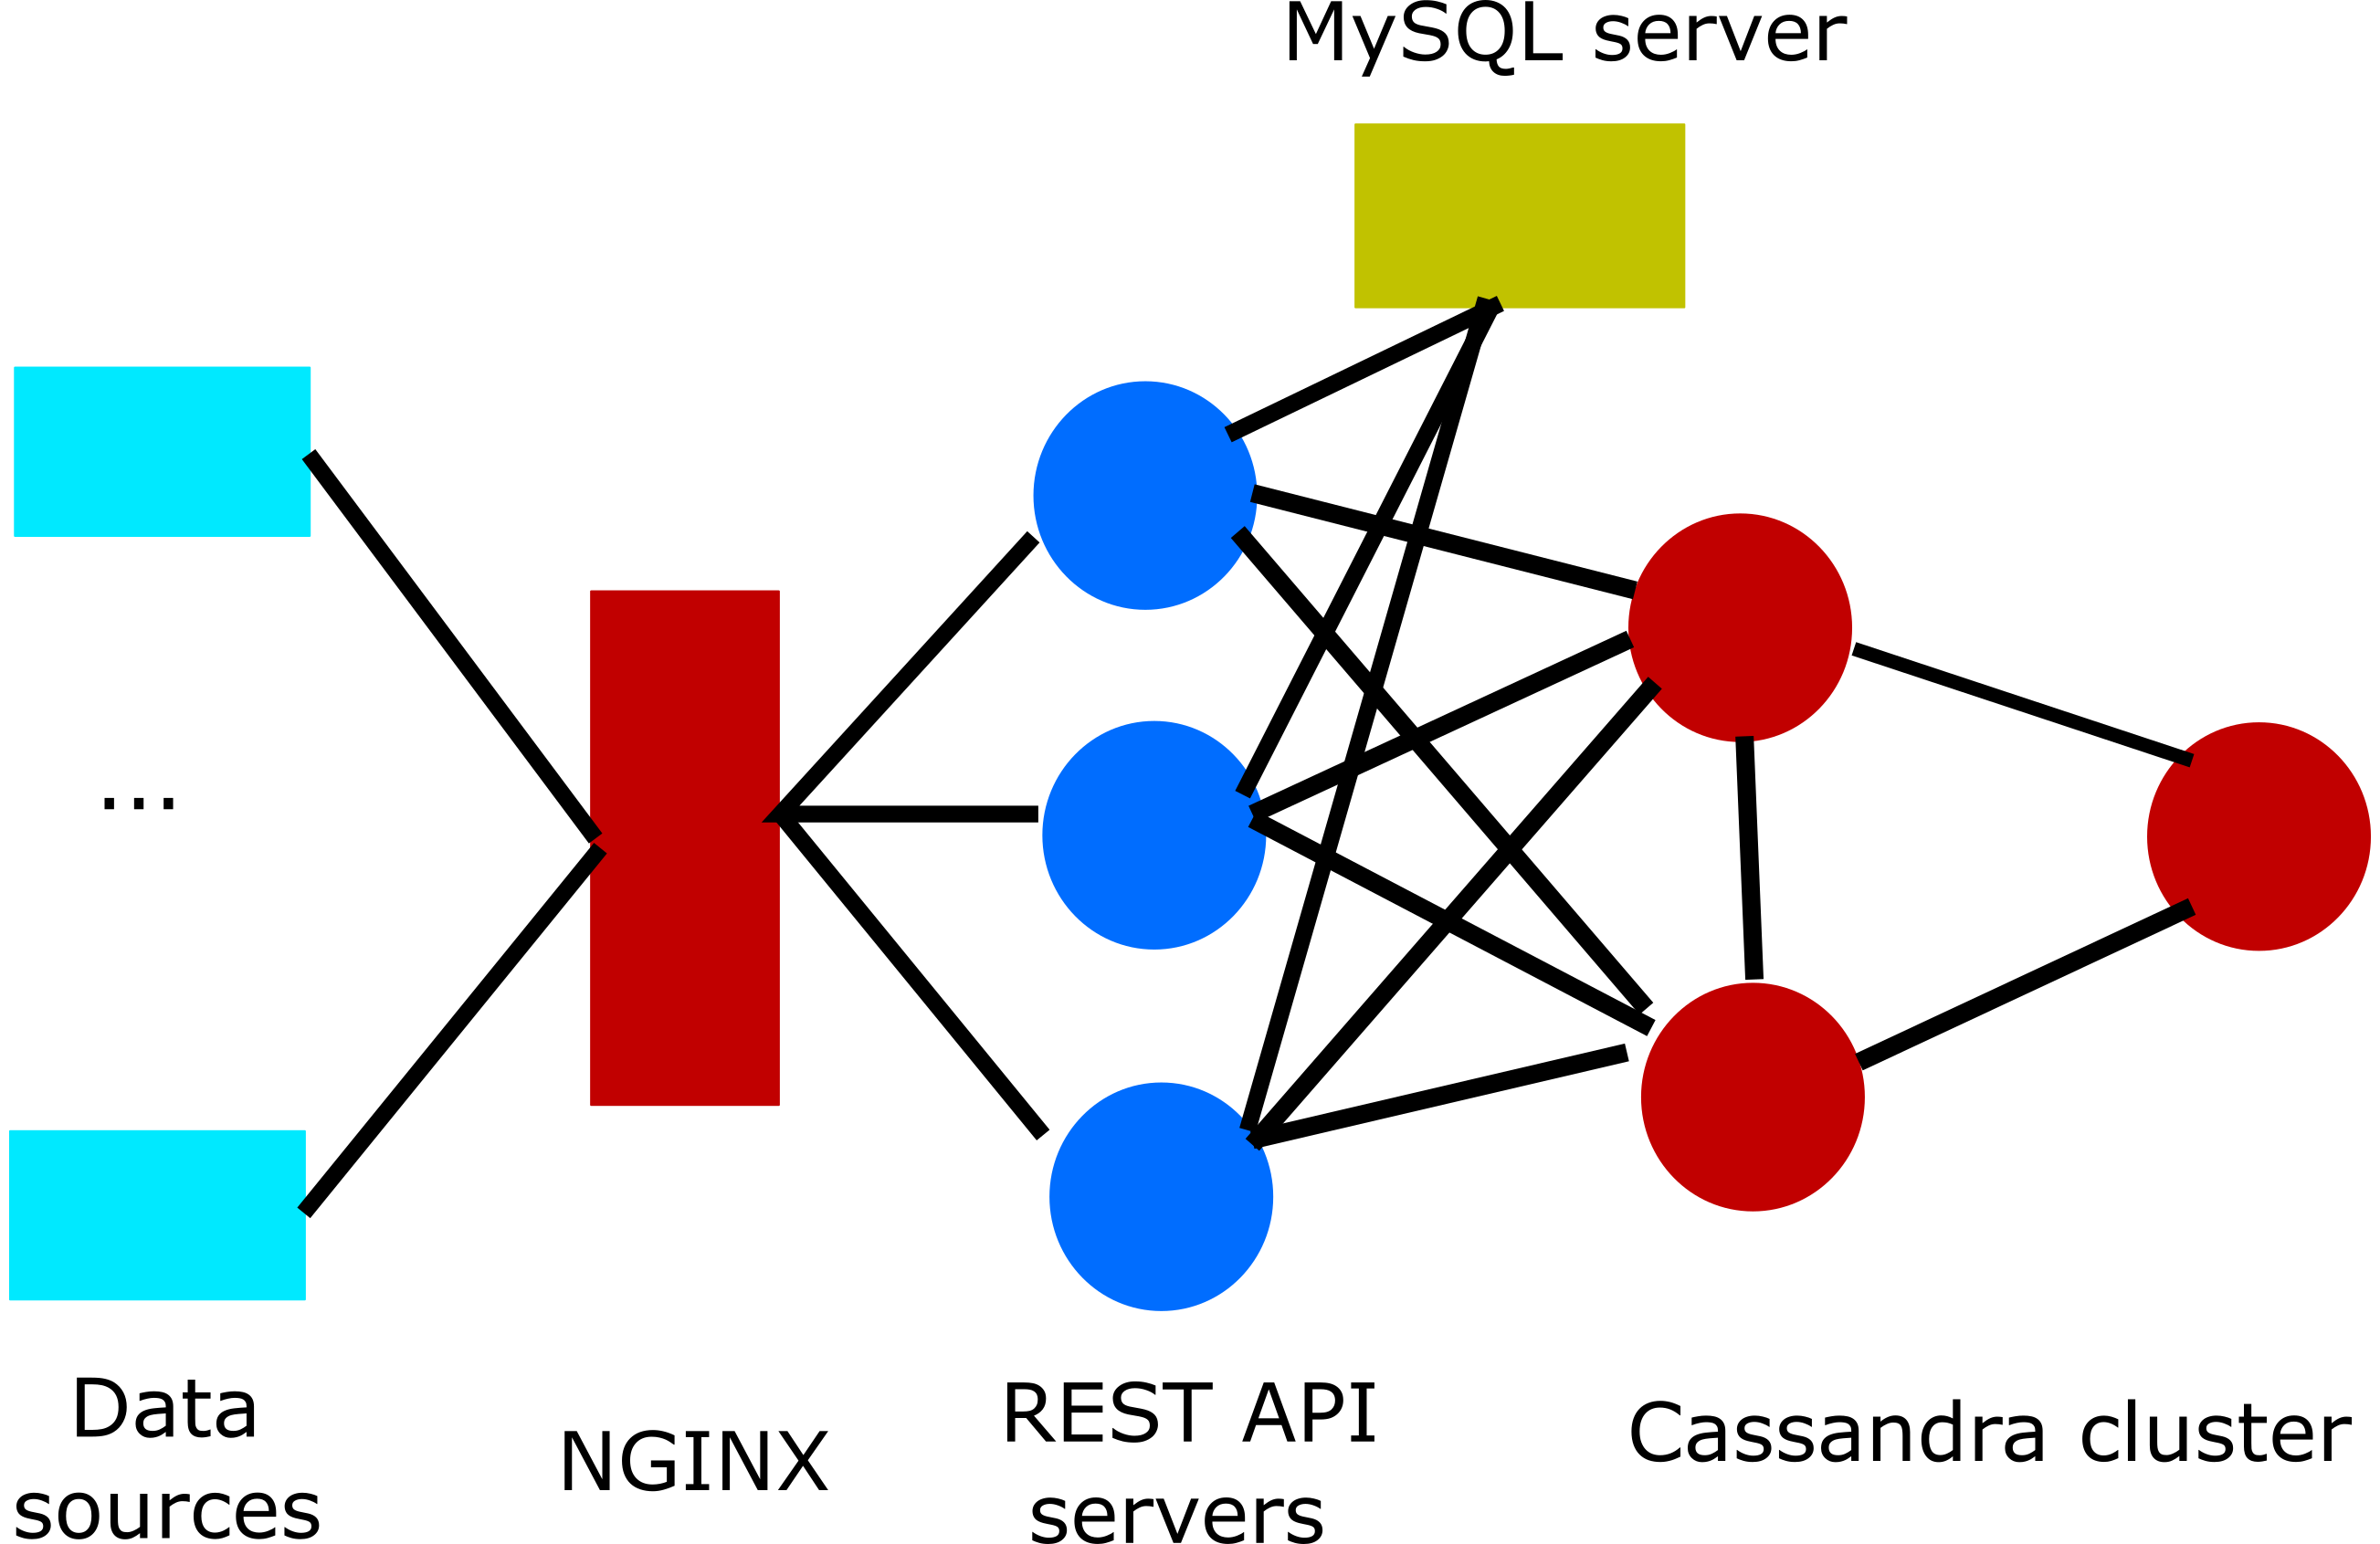
\includegraphics[width=0.45\textwidth]{graphics/arch.png}
  \caption{Process Historian Architecture}
  \label{fig:arch}
\end{figure}

The Cassandra row design is depicted in Figure~\ref{fig:schema}.
It is basically consists of a wide row (1 day long) and a composite
partition key: tag plus date bucket (date bucket splits the data 
into 1 day periods). The parameters for Cassandra 
clusters are shown in Table~\ref{tab:params}.

\begin{figure}[!hbt]\centering
  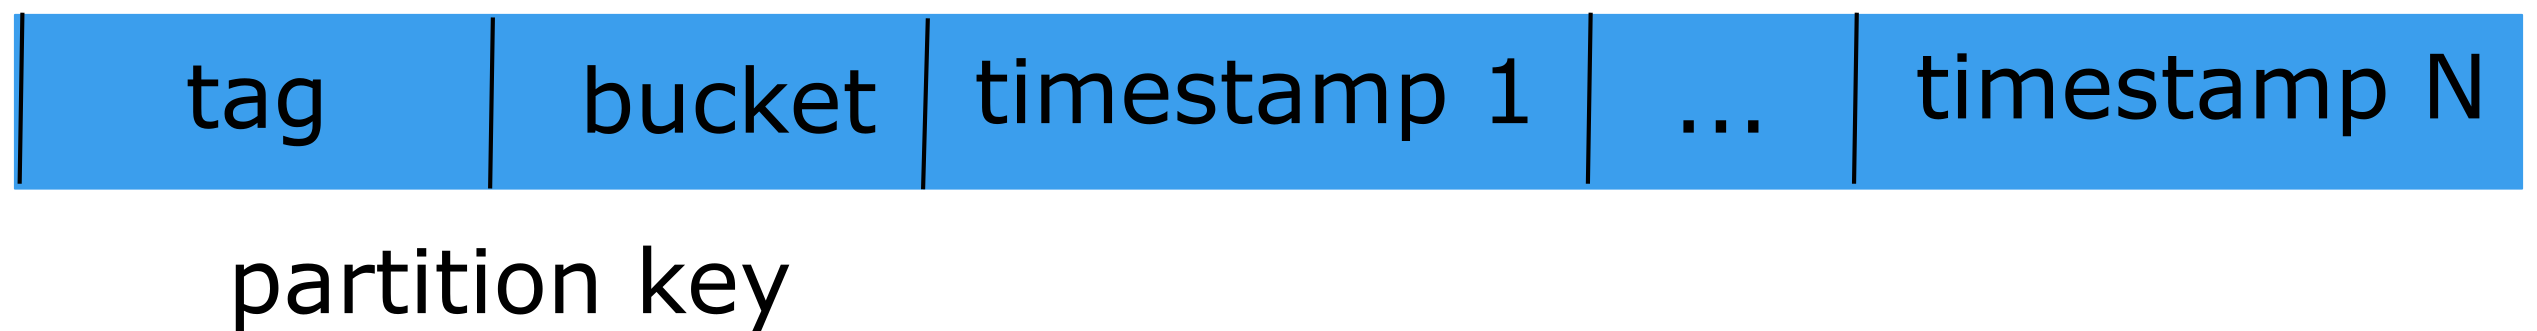
\includegraphics[width=0.45\textwidth]{graphics/schema.png}
  \caption{Cassandra schema design}
  \label{fig:schema}
\end{figure}


\begin{table*}[htp!]
  \caption{Cassandra parameters}
  \label{tab:params}
  \centering
  \begin{tabular}{lcc}
    \hline
    {\bf Parameter}                                  & {\bf Value } \\
    \hline
    Number of nodes in the cluster                   & 3       \\
    Replication factor                               & 2       \\
    Node RAM size                                    & 2 GB    \\
    TTL                                              & 1 year  \\
    Number of seed nodes                             & 1       \\
    Partitioner                                      & uniform (Murmur3Partitioner) \\
    Read and write consistency                       & quorum  \\
  \end{tabular}
\end{table*}

The remaining parameters where left unchanged and were configured
during the release of Cassandra 4.1.9 by the developers.

Overall, our MVP includes the implementation of the 
following functionality: (i) sensor metadata manipulation
(addition, removal, and modification of the sensor information
in the MySQL database), (ii) raw sensor data injection (we
have also implemented a simple authentication layer, according to which 
every data source was creating an HMAC for each tag (this information was 
verified at the REST API server using the secret key it shared
with particular sensor), (iii) raw sensor data
retrieval using tag name, start, and end periods for filtering.

We should note that it is rather trivial to also add data 
rollup, aggregation (such as finding mean, max, min, etc.)
and extrapolation (such as time-series prediction) features
into the code. But all this was out of the scope in this 
study. 

